\chapter{Results Analysis}

\section{Short Dated Puts and Calls}

The first test we performed involved all priced short-dated puts and calls for stocks on the Dow. Our test was run one business week prior to the expiry of the puts and calls and exported for analysis. For each of these, the simplest test we could use to determine the differences from actual values was a Sum Squared Error (SSE) test. The results are shown in table 3.1.

\begin{table}[h!]
\centering
\begin{tabu} to .8\textwidth { | X[c] | X[c] | }
 \hline
Method & Combined SSE (Puts + Calls)\\
 \hline
Barone-Adesi Whaley & 1633.569682 \\
Bjerksund-Stensland &  1633.67047532\\
Cox-Ross-Rubenstein & 1634.02600139 \\
Jarrow-Rudd & 1634.02313417 \\
Equal Probabilities & 1634.140215 \\
Trigeorgis & 1634.02323538 \\
Tian & 1634.02877159\\
Leisen-Reimer & 1633.9644903\\
\hline
\end{tabu}
\caption {\textbf{Combined SSE values from the one week expiry test.}}
\end{table}

As shown in the table, for the one-week test there is a very small difference observed between the estimation methods. This indicates that, at least for the one week dated options, no method has a guiding advantage over the other. This is not unexpected; due to the very small time to expiry, the potential values of each method?s random walk are less inclined to deviate heavily.

Diving further into the analysis, we elected to perform a threshold accuracy test which would give us a better idea of the values closeness to their intended value. For a threshold accuracy of 1 (that is, estimations were within \$1 of the actual price value, we saw that for put options each test typically 86\% of results fell within our expected range. This is quite good. Call options were less accurately priced, with roughly 75\% of modeled options falling within \$1 of expected price value. Still, neither were particularly poor representations.

We then elected to plot the actual prices versus the estimated model's results. This gave us a better indication of the model's tendencies in estimation. The following graphs were produced for the one week puts and calls of an AAPL (Apple Inc.) stock. 

\begin{center}
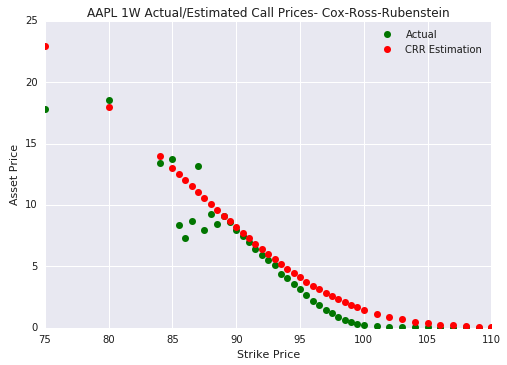
\includegraphics[scale=0.66, keepaspectratio=true]{Chapter3/CRRCall1W.png}
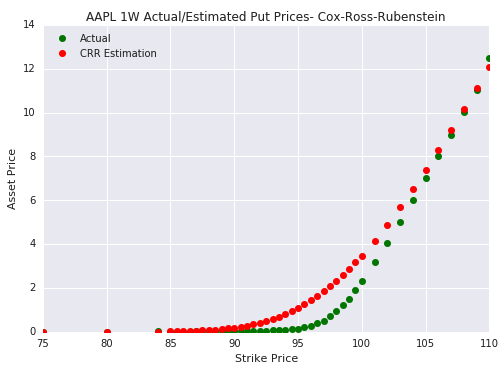
\includegraphics[scale=0.66, keepaspectratio=true]{Chapter3/CRRPut1W.png}
\end{center}

Both put and call charts indicate that our model seems to overestimate values. This is not necessarily unexpected, as results are generated entirely upon volatility. As we can see, however, in line with our previous threshold prediction values put prices are clearly more accurately priced. We also see that options with strike prices closer to the price of the share are much harder to predict. During these tests, AAPL shares were priced around \$98. 

With this test, however, no clear leading model in options pricing has made itself apparent. There also appears to be little difference experienced in using the binomial model as opposed to Black-Scholes and its variants.

\section{Long Dated Puts and Calls}

Since option prices vary more widely as times extend out further, tests also had to be run for longer times in order to determine their accuracy. An exipry date approximately six months in the future (January 2017) was selected. The analysis was then rerun for both sum squared error and threshold accuracy. 

\begin{table}[h!]
\centering
\begin{tabu} to .8\textwidth { | X[c] | X[c] | }
 \hline
Method & Combined SSE (Puts + Calls)\\
 \hline
Barone-Adesi Whaley & 41813.4995377\\
Bjerksund-Stensland &  41838.2751664\\
Cox-Ross-Rubenstein & 41777.9329279\\
Jarrow-Rudd & 41777.7318535 \\
 Equal Probabilities & 41817.923815\\
Trigeorgis & 41778.030902 \\
Tian & 41776.6236091\\
Leisen-Reimer & 41775.6888507\\
\hline
\end{tabu}
\caption {\textbf{Combined SSE values from the one month expiry test.}}
\end{table}


Once again, though, we see very little difference in the values considering the six month expiry date. This is unexpected.  The values deviate by less than one hundred in range. Looking at a threshold accuracy value, we see a pattern of decreased accuracy, at least when pricing calls. Only 17\% of calls were within \$1 of their actual values. Sixty-eight percent of puts were accurate within \$1. When increasing the threshold to \$5, the results were far better at 73\% of calls and 90\% of puts. Still, $\pm\$5$ is a very wide margin of error considering the prices of individual options contracts.

Expanding our analysis out, we'll once again look at our estimated prices for AAPL's six-month calls versus their real values. 

\begin{center}
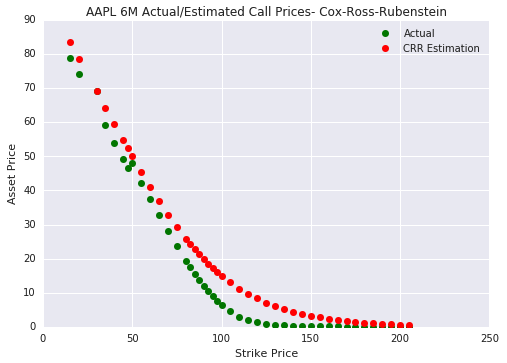
\includegraphics[scale=0.66, keepaspectratio=true]{Chapter3/AAPL6MCall.png}
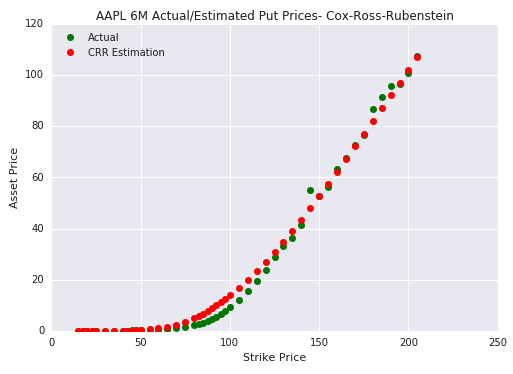
\includegraphics[scale=0.66, keepaspectratio=true]{Chapter3/AAPL6MPut.png}
\end{center}

These graphs indicate very fair valuations in the case of put options, and much poorer accuracy for call options. This was indicated early on by the SSE values for puts and calls. Typically, SSE values for all call option tests were around 24,000, while put options had SSE values of around 18,000. Returning to the graphs, we see greater inaccuracy for options with strike prices around the underlying asset values. 

Surprisingly, in these tests there is once again no model which clearly leads in accuracy. SSE values for each of the models were all grouped closely, and the only discernable difference in accuracy that could be found was the pricing of put or call options.

\section{Very Long Dated Puts and Calls}

After observing little difference in the accuracies of the models for six-month expiry puts and calls, we decided to attempt to price options with expiries almost one and a half years away from the current date. Pricing options for January 19, 2018, we saw the following SSE results:

\begin{table}[h!]
\centering
\begin{tabu} to .8\textwidth { | X[c] | X[c] | }
 \hline
Method & Combined SSE (Puts + Calls)\\
 \hline
Barone-Adesi Whaley & 92095.2212736\\
Bjerksund-Stensland &  92034.9437455\\
Cox-Ross-Rubenstein & 91944.8014098\\
Jarrow-Rudd & 91940.288989 \\
 Equal Probabilities & 92143.5437267\\
Trigeorgis & 91943.2074004 \\
Tian & 91929.01258\\
Leisen-Reimer & 91940.5065844\\
\hline
\end{tabu}
\caption {\textbf{Combined SSE values from the 1.5 year expiry test.}}
\end{table}

Even at a time to expiry of 1.5 years we still observe that the models remain relatively closely grouped in their accuracies. In fact, we observe a standard deviation in SSE values of around 83.8, which is very close grouping for numbers as high as these values are. This seems to suggest that in most cases we will see little variance in the results of our estimation methods. Not only that, it also seems to suggest that there is no particular reason to use the Black-Scholes model over the binomial (or vice-versa). 

Observing threshold accuracy, we see that 42\% of calls fall within one dollar of the actual values. Forty-five percent of puts fall within one dollar of their actual value. SSE values varied widely between puts and calls once again. In this case, however, SSEs for call values were six times those of put values, equating to around 79,000. Put values averaged SSEs of around twelve thousand. 

Graphing the data, we observe a picture similar to what we have seen in the two previous estimations. Note the difference between the estimated call prices and the actual call prices.

\begin{center}
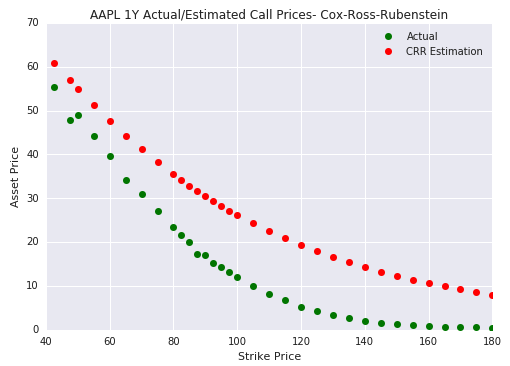
\includegraphics[scale=0.66, keepaspectratio=true]{Chapter3/AAPL1YCall.png}
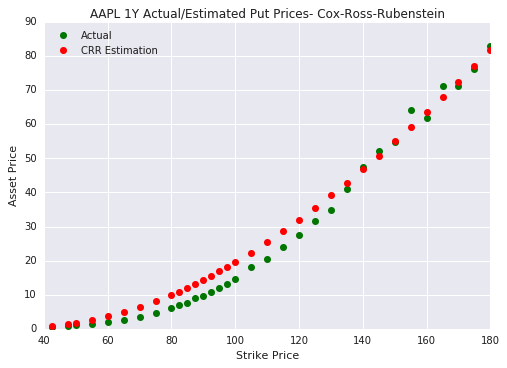
\includegraphics[scale=0.66, keepaspectratio=true]{Chapter3/AAPL1YPut.png}
\end{center}

In this situation, the AAPL put prices remain fairly stable and sensible. The call prices are off by very large amounts, as was suggested by our SSE calculations. This in turn seems to suggest that in the long run, both Black-Scholes and the Binomial method may overestimate the value of call returns.


